%
% File: introduction.tex
% Author: Eshwen Bhal
% Description: Introductory chapter.
%
\let\textcircled=\pgftextcircled
\chapter{Introduction}
\label{chap:intro}

\initial{T}he universe, in all its vastness, structure, natural laws and chaos, is comprised of only three principal components: visible matter, the ingredients of stars, planets and life, is the only one we interact with on a regular basis; dark energy, a force or manifestation of something even more mysterious, responsible for the accelerating expansion of the universe, is almost entirely unknown; and dark matter, a substance invisible in all sense of the word, that binds galaxy together and influences large scale structure in the cosmos, is the topic of this thesis.

\begin{easylist}[itemize]
\ListProperties(Style*=-- , FinalMark={)}, Margin=0.5cm)
& Describe dark matter. If the main talking points regarding motivation, evidence for its existence, etc. will be discussed in theory chapter, then only briefly describe here.
& Briefly outline particle accelerators and their function, the fact that we can use them to potentially discover dark matter or infer more of its properties, and the models that will be discussed in more detail to try and achieve this outcome.
& The introduction probably doesn't need to be too long, maybe only a few pages. Compare length with other people's theses (ask Ben Krikler for a copy of his, look at Alex's and Lana's).
\end{easylist}

%=======
\section{Section}
\label{sec:sec01}

Begins a section.

\subsection{Subsection}
\label{subsec:subsec01}

Begins a subsection.

%A figures matrix.
\begin{figure}[htbp]
\centering
\begin{minipage}{3.3cm}
    \centering
    \subtop[]{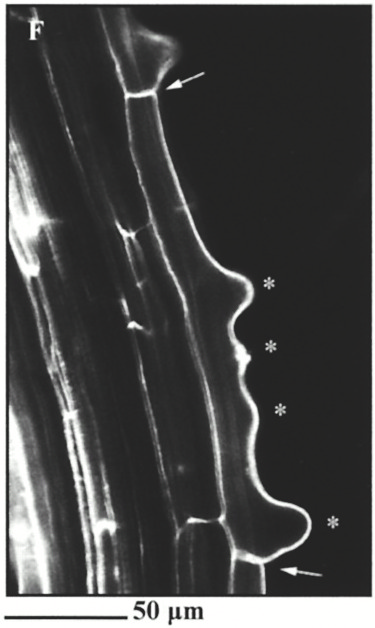
\includegraphics[height=0.28\textheight]{fig01/Nswellings}\label{sf:multiRH02a}}
\end{minipage}
\hspace{0.5cm}
\begin{minipage}{3.3cm}
    \centering
    \subtop[]{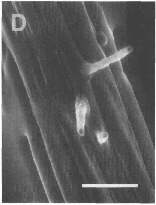
\includegraphics[height=0.27\textheight]{fig01/Mswellings}\label{sf:multiRH02b}}
\end{minipage}
\hspace{1.3cm}
\begin{minipage}{3.3cm}
    \centering
    \subtop[]{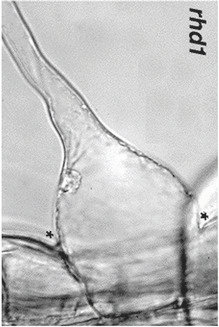
\includegraphics[height=0.27\textheight]{fig01/rhd1}\label{sf:multiRH02c}}
\end{minipage}
\\ \vspace{0.1cm}
\begin{minipage}{10cm}
    \centering
    \subtop[]{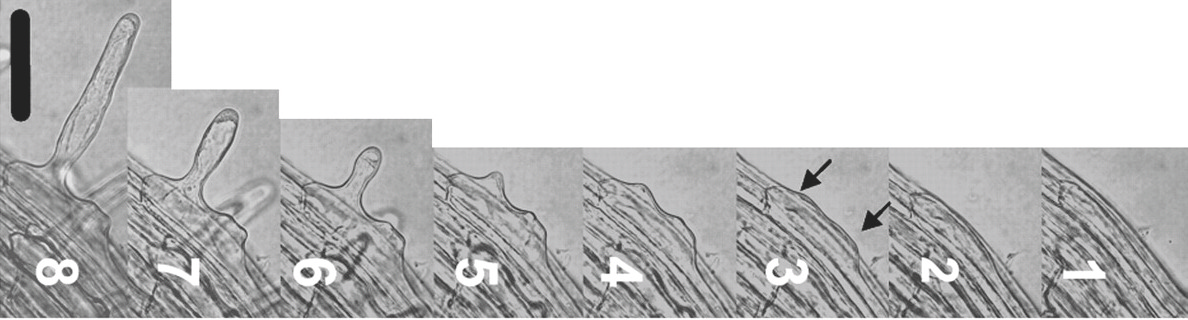
\includegraphics[height=0.145\textheight]{fig01/mutantrhd6}\label{sf:multiRH02d}}
\end{minipage}
\\ \vspace{0.1cm}
\begin{minipage}{10cm}
    \centering
    \subtop[]{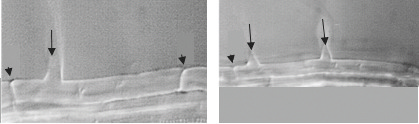
\includegraphics[height=0.16\textheight]{fig01/auxab}\label{sf:multiRH02e}}
\end{minipage}
\mycaption[Hair-forming mutant cells.]{(a) A mutant RH cell. Asterisks show multiple sites of RH initiation in a single root hair cell (indicated by the arrows). Figure reproduced from Ref.~\cite{rigas01}. (b)~Hair-forming cell with three RH initiation locations. The bar represents 50\,\si{\micro}m. Figure reproduced from Ref.~\cite{massuci01}. (c) Large bump in mutant {\itshape rhd1}. Figure reproduced from Ref.~\cite{griersonRH}. (d) Mutant overexpressing gene {\itshape ROP2}; from right-hand to left-hand, numbers indicate progressive snapshots at different times. RH initiation sites are indicated by the arrows. The bar represents 75\,\si{\micro}m. Figure reproduced from Ref.~\cite{mjones01}. (e)~Mutants affected by auxin. On the left-hand side, RH site is farther away from the apical end (left arrow cap); on the right-hand side, multiple RH locations (arrows). Figure reproduced from Ref.~\cite{payne01}.}
\label{fig:multiRH02}
\end{figure}

% A single figure
\begin{figure}[htbp]
	\centering
	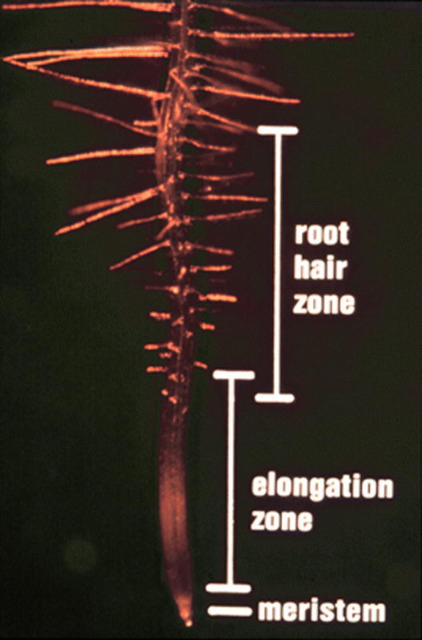
\includegraphics[height=0.35\textheight]{fig01/devepzones}
	\mycaption[Developmental zones of an Arabidopsis root.]{Developmental zones of an Arabidopsis root. Figure reproduced from \cite{griersonRH}.}
	\label{fig:RHP02}
\end{figure}

\newpage

Here is some text, just to check how it's displayed. blah blah blah blah blah blah blah blah blah blah blah blah blah blah blah blah blah blah blah blah blah blah blah blah blah blah blah blah blah blah blah blah blah blah blah blah blah blah blah blah blah blah blah blah blah blah blah blah blah blah blah blah blah blah blah blah blah blah blah blah blah blah blah blah blah blah blah blah blah blah blah blah blah blah blah blah blah blah blah blah 

\newpage

Doing the same to check both sides of the paper (for when it's bound).

Also testing glossaries: \gls{latex}, \acrlong{lhc}, \acrshort{lhc}, \acrfull{lhc}.

Also testing references: \cite{CMS-PAPER-SUS-15-005-published} (article), \cite{tagkey1984quarksandleptons} (book), \cite{Lisanti:2016jxe} (inproceedings), \cite{CMS-PAS-SUS-15-005} (techreport).

Testing numbers: 1234567890 (normal), $1234567890$ (math), \si{1234567890} (from siunitx).

Testing alphabet: The quick brown fox jumps over the lazy dog

Testing math characters compared to normal text: \Pqb-tag, $b$-tag, \emph{b}-tag, $\Pqb b\mathrm{b}\text{b}$\emph{b}b, $\Pqc c\mathrm{c}\text{c}$\emph{c}c.

Testing equations: $\sfrac{1}{2} \rho \Delta \phi \mathcal{L}$ (inline)
\begin{equation}
B(P) = \frac{\mu_0}{4\pi} \int \frac{I \times \hat{r}}{\bar{r}^2}\mathrm{d}r \ \text{(equation environment)}
\end{equation}

Testing symbols/macros: \eV, \MeV, \GeV, \TeV, \pt, \ptmiss, \met, \HT, \mht, \mt, \aDark, \rinv, \mqdark, \doubleMuCr, \doubleLepMass, \alphat, \ttbarpjets, \wtolnupjets, \LSP.

%=========================================================